\section{Data Generation}

Before models for the detection of mechanical symbols can be created, it is necessary to collect data suitable for this task.

The aim is to read handwritten mechanical symbols.
The data for training the model are necessarily created by myself at this point.
Since the data generation can be time consuming, a way had to be found to create the data as time efficient as possible.
Fortunately I had access to a tablet which allows to draw directly on the display.
To generate the data quickly, some requirements had to be taken into account:
\begin{enumerate}
    \item A drawing context is created.
    \item The context is variable in size and color.
    \item The context should be able to recognize mouse events.
    \item The script should have access to the file system to safe data on the hard drive with no extra work required.
\end{enumerate}

A Python script is able to meet these requirements.
The library \name{OpenCV} \cite{OpenCV2019} allows to create a window with corresponding requirements. The library \name{opencv-python} \cite{Heinisuo2019} is used here implementation of \name{OpenCV}.
It meets all these requirements because it provides the creation of a window with programmable context and functions to handle mouse events\footnote{The data generation should be done using JavaScript in a web context, but the final requirement to secure data does not seem to be easy to meet. Node.js has access to the filesystem, but is inherently "headless" and therefore does not allow any context to be used for drawing. }.

Since the model should be able to recognize symbols of any color on any background, the context background is a random value in grayscale, as is the color of the line drawn on the background.
The thickness of the line used for drawing is also random, thus mimicking the appearance of a symbol of different sizes\footnote{This should serve to predict images of different resolutions in a later process}.

After the parameters used to draw the context have been set, the function \name{cv2} is used to \code{namedWindow} created the function \name{cv2}. 
For each interaction with the canvas, the \code{setMouseCallback} function is applied to the generated \code{namedWindow}, calling a \code{draw} function that allows to detect and react to mouse events.

Drawing is done by functions triggered by events called \code{cv2.EVENT\_LBUTTONDOWN} and \code{cv2.EVENT\_LBUTTONUP}, which set a boolean \code{drawing} flag to either \code{True} or \code{False}.
The drawn image is saved with \code{cv2.Event\_RBUTTONUP}, which names the image after the number of previously automatically drawn images.

The names of the different classes are set at the beginning of the script, with an interactive prompt asking the user which class to fill next, with the options \textit{"x" for base, "o" for link, "n" for no match}.
Consideration of \textit{not found} is especially important because later, when searching for any image, most responses are likely to contain no symbol at all.

With this script 500 symbols are created for each class.
It is expected that these images will be augmented later to counteract overfitting, but for the task of distinguishing three different classes, this set should be sufficient\footnote{The code can be viewed at \aka{https://github.com/klawr/deepmech/tree/master/reports/srp/code/data_generation.py}}.

\begin{figure}
    \centering
    \begin{subfigure}[b]{0.3\textwidth}
        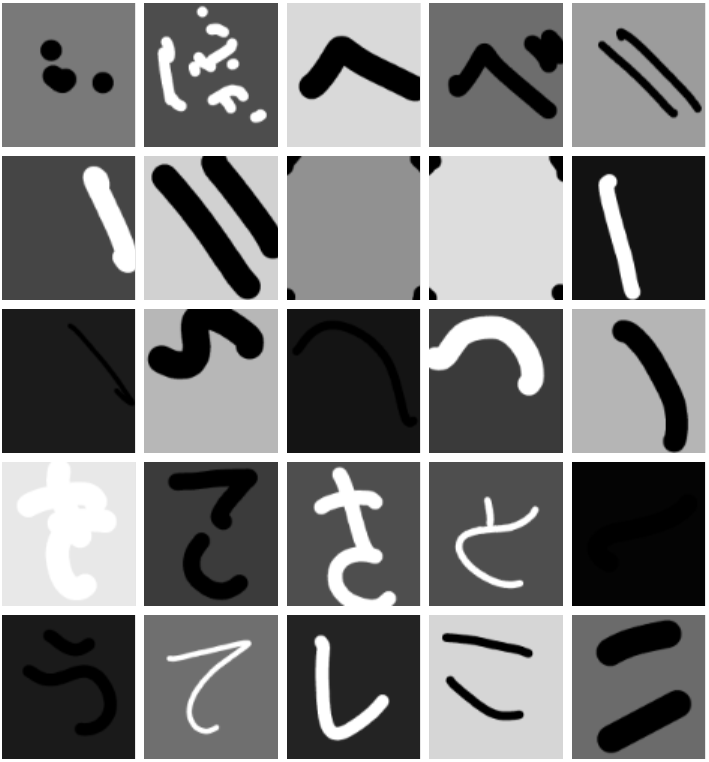
\includegraphics[width=\textwidth]{images/25_n.png}
        \caption{Non hits}
        \label{fig:25_non_hits}
    \end{subfigure}
    \begin{subfigure}[b]{0.3\textwidth}
        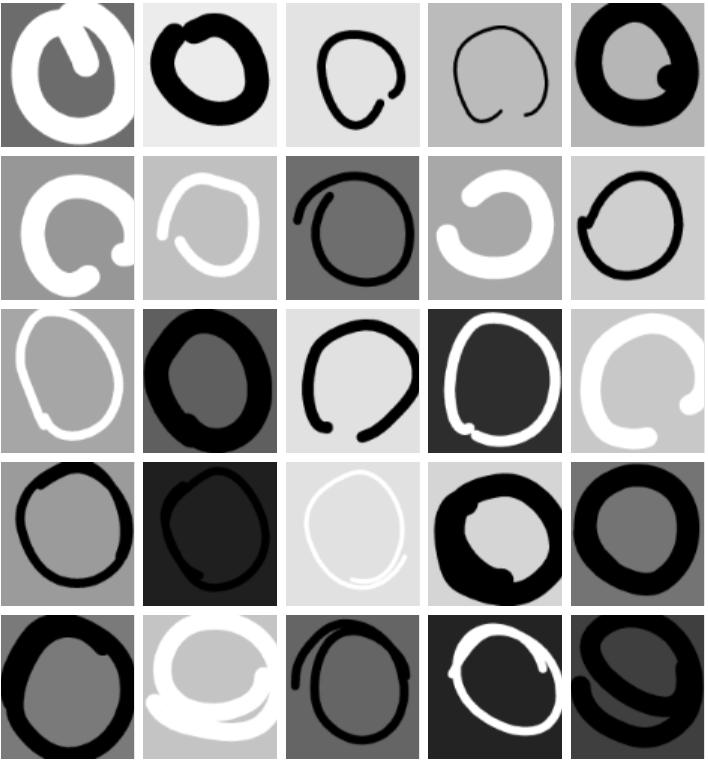
\includegraphics[width=\textwidth]{images/25_o.png}
        \caption{Nodes}
        \label{fig:25_links}
    \end{subfigure}
    \begin{subfigure}[b]{0.3\textwidth}
        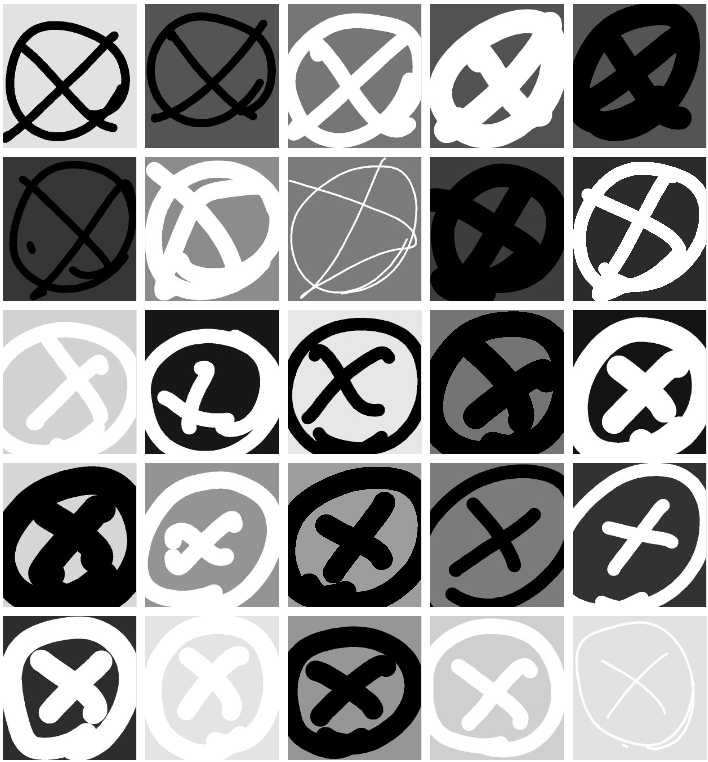
\includegraphics[width=\textwidth]{images/25_x.png}
        \caption{Bases}
        \label{fig:25_bases}
    \end{subfigure}
    \caption[Examples of node data for training]{Some examples of the data created with the described method. Only these three classes were created for the first tests. The images are created centered in a square, so that later any images can be scanned, using squares of different sizes as templates. }
    \label{fig:generated_data_samples}
\end{figure}
